
\documentclass[aspectratio=169]{beamer}
\usetheme{metropolis}           % Use metropolis theme
\usepackage[utf8]{inputenc}
\usepackage{graphicx}
\usepackage{eso-pic}
\usepackage{graphics}
\usepackage{tikz}
\usepackage[export]{adjustbox}
\usepackage{multicol}
\usepackage{listings}
\usepackage{helvet}
\usepackage{booktabs}
\usepackage{threeparttable}
\usepackage{fontspec}
\usepackage{hyperref}
\hypersetup{urlcolor=DarkBlue}

\title{Stata Track 1 - Topic 3 \newline In-Field Data Quality Checks}
\date{\today}
\author{Luiza Andrade, Kristoffer Bjarkefur} % Name of author(s) of session here
\institute{Development Impact Evaluation (DIME) \newline The World Bank }
\setbeamercolor{background canvas}{bg=white}	% Sets background color

% The below command places the World Bank logo and DIME logo to the right corner
\titlegraphic{%
	\begin{picture}(0,0)
	\put(330,-180){\makebox(0,0)[rt]{
\includegraphics[width=3cm]{../../img/WB_logo}}}
	\end{picture}%
	\begin{picture}(0,0)
	\put(390,-180){\makebox(0,0)[rt]{
\includegraphics[width=1.5cm]{../../img/i2i}}}
	\end{picture}%
}

%%% Section page with picture of Light bulb
\makeatletter
\defbeamertemplate*{section page}{mytheme}[1][]{
	\centering
	\begin{minipage}{22em}
		\raggedright
		\usebeamercolor[fg]{section title}
		\usebeamerfont{section title}
		\par
		\ifx\insertsubsectionhead\@empty\else%
		\usebeamercolor[fg]{subsection title}%
		\usebeamerfont{subsection title}%
		\fi
		\ifstrempty{#1}{}{%
			\includegraphics[width=100mm, height=60mm]{#1}%
		}
		\insertsectionhead\\[-1ex]
		\insertsubsectionhead
		\usebeamertemplate*{progress bar in section page}

	\end{minipage}
	\par
	\vspace{\baselineskip}
}
\makeatother

%%% Define a command to include picture in section,
%%% make section, and revert to old template
\newcommand{\sectionpic}[2]{
	\setbeamertemplate{section page}[mytheme][#2]
	\section{#1}
	\setbeamertemplate{section page}[mytheme]
}

\usepackage{fancyvrb} % Allows customization of verbatim environments
%Fancyvrb docs: http://mirrors.ibiblio.org/CTAN/macros/latex/contrib/fancyvrb/doc/fancyvrb-doc.pdf
\fvset{fontsize=\scriptsize} % The font size of all verbatim text can be changed here

%So we can use option FloatBarrier, which is similar to [H] but is an
%alternative solition when the algorithm can't solce [H] as too many
%settings are going on. [H] seems to get stuck in infinite loop
%https://tex.stackexchange.com/questions/2275/keeping-tables-figures-close-to-where-they-are-mentioned
\usepackage{placeins}
\newcommand{\codeexample}[2]{
	\begin{figure}
		\VerbatimInput[
		framesep=3mm,
		frame=lines, % line above and below code section
		numbers=left, %Line number
		label= #1, %name of code section
		baselinestretch=0.90, %Use line space more similat to line space in code editors
		]{#2} %Write the relative file path and the name of the file to be included
	\end{figure}
	\FloatBarrier
}

%% The below command creates the ligh bulb logos in the top right corner of the
\begin{document}

	{
		\usebackgroundtemplate{
\includegraphics[height=55mm, right]{../../img/top_right_corner.pdf}}
		\maketitle
	}

%%%%%%%%%%%%%%%%%%%%%%%%%%%%%%%%%%%%%%%%%%% heading of section 1
\begin{frame}{Objectives}
	\begin{itemize}
		\item Duplicates
		\begin{itemize}
			\item Run a prepared file using \texttt{ieduplicates} command and understand the output
			\item \texttt{Purpose:} Make sure you can identify the respondent while the enumerator still remember the interview
		\end{itemize}
		\item Survey Log / Progress Report
		\begin{itemize}
			\item List the number of completed interviews
			\item \texttt{Purpose:} Make sure we are making enough progress to complete sample before money runs out
		\end{itemize}
		\item High Frequency Checks (HFC)
		\begin{itemize}
			\item Download and use IPA's framework for HFCs
			\item \texttt{Purpose:} Make sure we are collecting data without a lot of errors reducing the quality of the data
		\end{itemize}
	\end{itemize}
\end{frame}

%%%%%%%%%%%%%%%%%%%%%%%%%%%%%%%%%%%%%%%%%%%
\sectionpic{Duplicates}{../../img/section_slide}

\begin{frame}{Why do we have duplicates?}
	\begin{itemize}
		\item To develop a quick but still secure way of dealing with any issue, we must first have a model for understanding the reasons that cause this issue
		\item Once we have a good model of the reasons for the issue, we will be able to develop a good methodology for how to solve the issues
		\item What type of reasons do we have for the duplicates in the ID variable we find in primary data?
	\end{itemize}
\end{frame}

\begin{frame}{Why do we have duplicates?}
	\begin{itemize}
		\item Type 1 - Double submissions of same observation and the same data
		\begin{itemize}
			\item First upload from tablet not complete due to bad internet
		\end{itemize}
		\item Type 2 - Double submissions of same observation but with modified data.
		\begin{itemize}
			\item Answers modified after submission, and then re-submitted
			\item Bad practice, more transparent to write correction in a do-file
			\item Many survey software have features preventing this.
		\end{itemize}
		\item Type 3 - Incorrectly assigned ID. Two respondents are given the same ID
		\begin{itemize}
			\item Typo in field when entering respondent ID
		\end{itemize}
	\end{itemize}
\end{frame}

\begin{frame}{How can we identify the types of duplicates?}
	\begin{itemize}
		\item Type 1 - Double submissions of same observation and the same data
		\begin{itemize}
			\item Few variables differs between the duplicates and differences are in submission data
			\item (\texttt{submission data} = submission time, submission ID, file attachment name etc.)
		\end{itemize}
		\item Type 2 - Double submissions of same observation but with modified data.
		\begin{itemize}
			\item Some variables differs between the duplicates and some of them are in observation data
			\item (\texttt{observation data} = age of respondent, professional occupancy, marital status, crops grown, what did you eat yesterday etc.)
		\end{itemize}
		\item Type 3 - Incorrectly assigned ID. Two respondents are given the same ID
		\begin{itemize}
			\item Many variables differs between the duplicates and many of the differences are in observation data
		\end{itemize}
	\end{itemize}
\end{frame}

\begin{frame}{ieduplicates}
	
	Wouldn't it be great if there was an command in Stata that would identify all duplicates and provide you with the information needed to determine which type it is?

	\begin{itemize}
		\item We have written: \texttt{ieduplicates}
		\begin{itemize}
			\item Part of the \texttt{iefieldkit} package. Installation \texttt{ssc install iefieldkit}
			\item Used in Stata but generates a report in Excel that team members not proficient in Stata can interact with
			\item The report is interactive, so you write your corrections in the Excel report, and the command will then apply those corrections
			\item Returns the data without the duplicates until they are solved
		\end{itemize}
	\end{itemize}
\end{frame}

\begin{frame}{ieduplicates - output}
	\begin{figure}
		\centering
		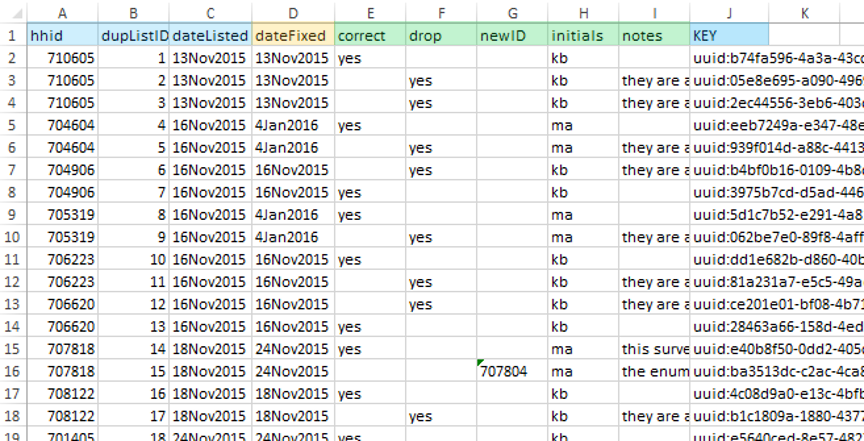
\includegraphics[width=.9\linewidth]{img/ieduplicates-output.png}
	\end{figure}
\end{frame}

\begin{frame}{ieduplicates - output}
	Attend the hands-on session on \texttt{ieduplicates} and \texttt{ietestform} to learn the details on how to best use \texttt{ieduplicates}. We will introduce some new features that were released only last month!
\end{frame}

%%%%%%%%%%%%%%%%%%%%%%%%%%%%%%%%%%%%%%%%%%%
\sectionpic{Survey Log}{../../img/section_slide}



\begin{frame}{Survey Log / Progress Report}
	\begin{itemize}
		\item Make sure to keep records in the field that is updated very day with how many interviews that were completed
		\item Make sure that the number of observations on the server matches these records.
		\item Purpose:
		\begin{itemize}
			\item Provide your team a quick overview of progress on the field
			\item Detect enumerators who are slacking
			\item Check balance if this is important for the survey (e.g. by gender)
		\end{itemize}
	\end{itemize}
\end{frame}


\begin{frame}{Survey Log / Progress Report}
	\begin{itemize}
		\item The HFC framework we will introduce next has a build in progress report, so we do not need to set this up separately. 
		\item The reason we are talking about this separately is that this test a slightly different thing than data quality and it is often forgotten in case it is not thought of as a step of its own.
	\end{itemize}
\end{frame}

%%%%%%%%%%%%%%%%%%%%%%%%%%%%%%%%%%%%%%%%%%%
\sectionpic{HFC}{../../img/section_slide}

\begin{frame}
	\begin{itemize}
		\item We are recommending IPA's (Innovation for Poverty Action \url{http://poverty-action.org}) framework for high frequency checks. 
		\begin{itemize}
			\item \url{https://github.com/PovertyAction/high-frequency-checks}
		\end{itemize}
		\item Like anything technical, there is a fixed cost to learn how to use
		\begin{itemize}
			\item However, if you are in the profession of primary data collection through surveys, then you need to learn or set up your own system for HFC. 
			\item This is the easiest to learn system that include the most number of features that we have come across, and it is definitely easier than setting up your own system of the same level of quality.
		\end{itemize}
	\end{itemize}
\end{frame}

\begin{frame}{IPA's HFC Framework}
	\begin{itemize}
		\item We will not have time to cover all features today, so we will cover a few examples of what we find most useful and important
		\item You should explore all the other features in this frame work after you feel comfortable with these basic examples.
	\end{itemize}
\end{frame}

\begin{frame}{Installing IPA's HFC Framework}

	Go to \url{https://github.com/PovertyAction/high-frequency-checks\#installation} and follow the installation instructions
	
	\vspace{.5cm}
	
	If you run in to errors (especially on a World Bank computer), let us know!

\end{frame}

\begin{frame}{Installing IPA's HFC Framework}

	If you for any reason cannot install with \texttt{net install} using an URL (the case on World Bank computers) you can do the following:
	\begin{itemize}
		\item Go to \url{https://github.com/PovertyAction/high-frequency-checks} and click the \texttt{Clone or download} button and select \texttt{Download ZIP}.
		\item You only need these files temporary so save them in your downloads folder or desktop and then un-zip the file and find the folder called \texttt{ado} in it. 
		\item Copy the file path to that ado folder and use that instead of the URL instead, see code example below.
		\item After you done this you can delete the zip file and the unzipped folders
	\end{itemize}

	\codeexample{install-from-local-pkg.do}{code/install-from-local-pkg.do}

\end{frame}


\begin{frame}{IPA's HFC: Folder set-up}

	Then set up a folder for this exercise and create a global for that folder. And after that run the set up command \texttt{ipacheck} to that folder. You can use any name in the option \texttt{surveys()}
	
	\codeexample{set-up-hfc.do}{code/set-up-hfc.do}
	
	If this does not work, you can unzip the zip file provided for this session. You still need to create teh folder global.

\end{frame}


\begin{frame}{IPA's HFC: Check folder set-up}

	Before continuing make sure you have a folder set-up inside you folder that looks like this:

	\begin{figure}
		\centering
		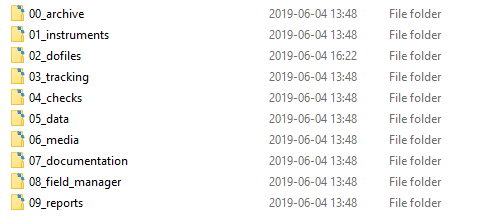
\includegraphics[width=.6\linewidth]{img/ipacheck-folders.png}
	\end{figure}

	Explore the folders. Inside the folders you will find text files that describe the purpose of each folder. We will in this exercise only use \texttt{02\_dofiles}, \texttt{04\_checks}, and \texttt{05\_data}.

\end{frame}

\begin{frame}{IPA's HFC: Use folder global in master\_check}

	Next, open up the do-file \texttt{02\_dofiles/master\_check.do}. Find the section shown below and add your folder global to the file path like the example below. Do not run the file yet.
	
	\codeexample{use-global-in-mastercheck.do}{code/use-global-in-mastercheck.do}

\end{frame}

\begin{frame}{IPA's HFC: Use folder global in master\_check}
	\begin{columns}[c]
	
		\column{.28\linewidth}
		\small Also in \texttt{master\_check.do} find this section and comment it out, i.e. add the two lines with \texttt{HERE}, line 2 and 20.
		
		\vspace{.2cm}
		
		\small There is nothing wrong with this section, the advanced version of the progress report is just out of the scope of this exercise to set it up.
	
		\column{.68\linewidth}
		\codeexample{progreport-not-use.do}{code/progreport-not-use.do}
	\end{columns}
\end{frame}

\begin{frame}{IPA's HFC: Use folder global in master\_check}
\begin{columns}[c]
	
	\column{.23\linewidth}
	\small Similarly, still in \texttt{master\_check.do} find this section and comment it out, i.e. add the two lines with \texttt{HERE}, line 4 and 11.
	
	\column{.73\linewidth}
	\codeexample{dups-not-use.do}{code/dups-not-use.do}
\end{columns}
\end{frame}


\begin{frame}{IPA's HFC: Set-up hfc\_inputs.xlsm}
	
	\begin{columns}[c]
		
		\column{.22\linewidth}
		\small Next, open up the excel file \texttt{hfc\_inputs.xlsm} in \texttt{02\_checks/01\_inputs}. 
		
		\vspace{.2cm}
		
		Go to the sheet called \texttt{0. Setup}. And copy these settings:
		
		\column{.78\linewidth}
		\begin{figure}
			\centering
			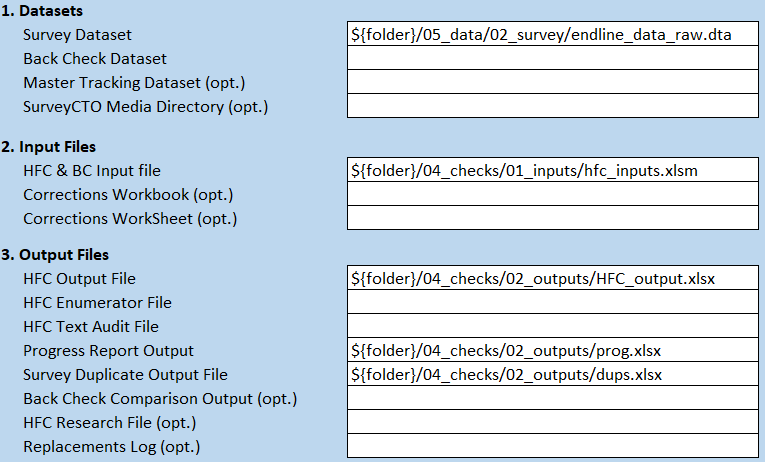
\includegraphics[width=\linewidth]{img/ipacheck-setup-1.png}
		\end{figure}
	\end{columns}
\end{frame}


\begin{frame}{IPA's HFC: Set-up hfc\_inputs.xlsm}
	\begin{columns}[c]
		
		\column{.22\linewidth}
		\small Then copy these settings:
		
		\column{.78\linewidth}
		\begin{figure}
			\centering
			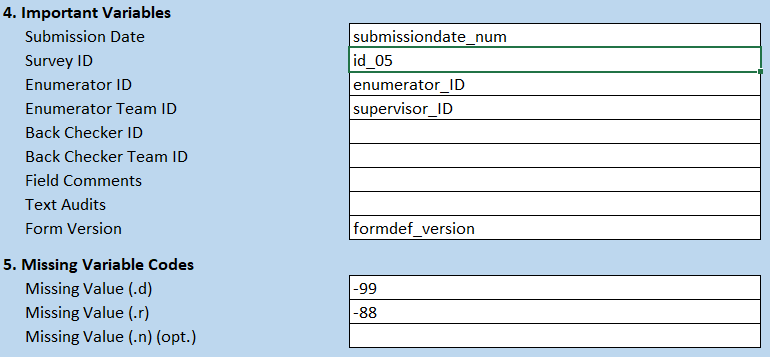
\includegraphics[width=\linewidth]{img/ipacheck-setup-2.png}
		\end{figure}
	\end{columns}
\end{frame}

\begin{frame}{IPA's HFC: Set-up hfc\_inputs.xlsm}
	\begin{columns}[c]
		
		\column{.22\linewidth}
		\small And then copy these settings:
		
		\column{.78\linewidth}
		\begin{figure}
			\centering
			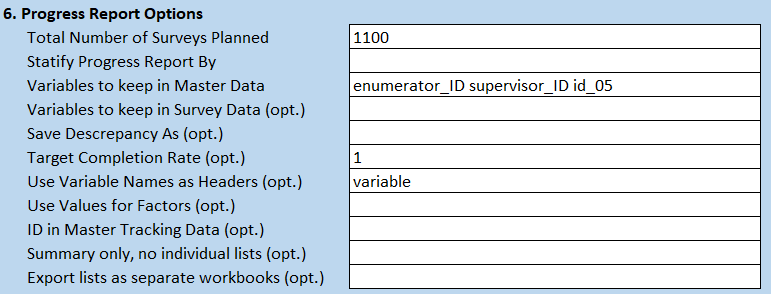
\includegraphics[width=\linewidth]{img/ipacheck-setup-3.png}
		\end{figure}
	\end{columns}
\end{frame}

\begin{frame}{IPA's HFC: Set-up hfc\_inputs.xlsm}
	\begin{columns}[c]
		
		\column{.22\linewidth}
		\small And finally make sure that only these options are checked:
		
		\column{.78\linewidth}
		\begin{figure}
			\centering
			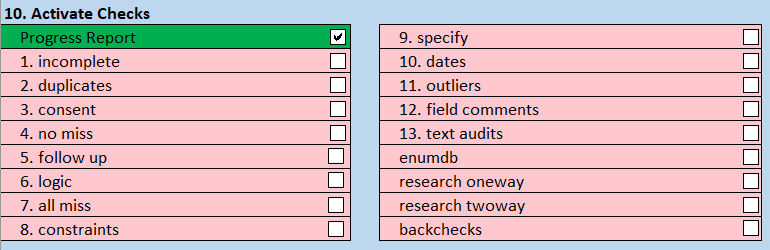
\includegraphics[width=\linewidth]{img/ipacheck-setup-4.png}
		\end{figure}
	\end{columns}
\end{frame}

\begin{frame}{IPA's HFC: Run the test}

	\begin{itemize}
		\item As the very last step copy the data set \texttt{endline\_data\_raw\_nodups.dta} to the folder \texttt{05\_data/02\_survey}. 
		\item Then after you have closed the Excel file, go back to \texttt{master\_check.do} and run the file!
		\item After the file is done running (could take a few moments), check out the two files that are created in the folder \texttt{04\_checks/02\_outputs}
	\end{itemize}
\end{frame}

\begin{frame}{IPA's HFC: Add no-miss test}

	\begin{itemize}
		\item \small Now open the \texttt{02\_checks/01\_inputs/hfc\_inputs.xlsm} again and go to the sheet called \texttt{4. no miss}.
		\item \small In the variable column, on separate rows, add the two variables \texttt{longitude} and \texttt{latitude}, and then in the \texttt{0. setup} sheet, select no miss like in the image below
		\item \small Coordinates of the respondents dwelling is an example of a variable we want to never be missing.
		\item \small Then run the \texttt{master\_check.do} and check \texttt{02\_checks/02\_outputs/HFC\_output.xlsm} 
	\end{itemize}

	\begin{figure}
		\centering
		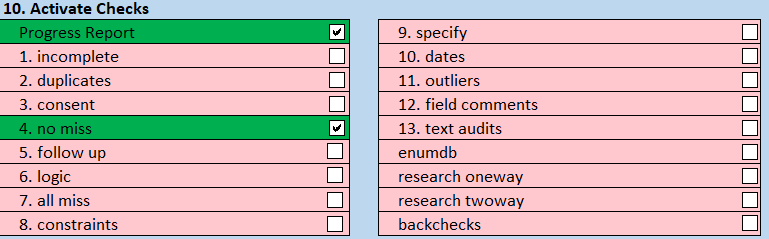
\includegraphics[width=.75\linewidth]{img/ipacheck-setup-nomiss.png}
	\end{figure}
\end{frame}

\begin{frame}{IPA's HFC: Add more tests}
	\begin{itemize}
		\item \small Now open the \texttt{02\_checks/01\_inputs/hfc\_inputs.xlsm} again and go to the sheet called \texttt{4. no miss}.
		\item \small In the variable column, on separate rows, add the two variables \texttt{longitude} and \texttt{latitude}, and then in the \texttt{0. setup} sheet, select no miss like in the image below
		\item \small Coordinates of the respondents dwelling is an example of a variable we want to never be missing.
		\item \small Then run the \texttt{master\_check.do} and check \texttt{02\_checks/02\_outputs/HFC\_output.xlsm} 
	\end{itemize}
\end{frame}



\begin{frame}{IPA's HFC: Add more tests}
	Do all of the next steps in \texttt{02\_checks/01\_inputs/hfc\_inputs.xlsm}
	\begin{itemize}
		\item In \texttt{6. logic}, add \texttt{crp\_08\_0\_1\_1\_1 amount\_harvest\_1\_1\_1} in the variable column, \texttt{!missing(crp\_08\_0\_1\_1\_1)} in the assert column, and \texttt{amount\_harvest\_1\_1\_1 == 0} in the if-statement column.
		\item In \texttt{7. all miss}, replace \texttt{\_all} with \texttt{health\_report\_01}, \texttt{health\_report\_02},..., \texttt{health\_report\_05}, 01-05 in the variable column. \texttt{\_all} would include all variables which is sometimes very useful, but some survey (like our example) has repeat patterns that create a lot of variables with all missing.
		\item In \texttt{8. constraints}, add all \texttt{pl\_age\_1},\texttt{pl\_age\_2},...,\texttt{pl\_age\_15}, 01-15, and 0 as \texttt{hard\_min} and \texttt{soft\_min}, 90 as \texttt{soft\_max} and 150 as \texttt{hard\_max},
		\item In \texttt{11. outliers}, add all the \texttt{inc\_1},\texttt{inc\_2},...,\texttt{inc\_17} variables. See that both variable and multiplier is green so both are required. Set all multipliers to 3.
	\end{itemize}
\end{frame}

\begin{frame}{IPA's HFC: Add more tests}	
	\begin{itemize}
		\item Then go to the \texttt{0. setup} sheet and select all tests we are now using (see image below)
		\item Then run the \texttt{master\_check.do} and check \texttt{02\_checks/02\_outputs/HFC\_output.xlsm} again.
	\end{itemize}
	
	\begin{figure}
		\centering
		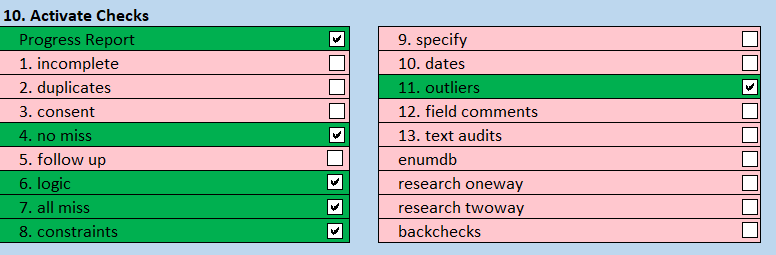
\includegraphics[width=.75\linewidth]{img/ipacheck-setup-add4.png}
	\end{figure}
\end{frame}

\begin{frame}{Finals notes on HFC}
	\begin{itemize}
		\item While manually coded HFC checks created by the project team will always be more specific to your project then an off-the-shelf framework will ever be, the main advantages of using an established framework like IPA's is that it reduces the risk that you forget to include a common and important test.
		\item You should explore the other tests in IPA's framework. It offers an impressive amount of flexibility.
		\item Once you learn to set up IPA's framework quickly, then you will have time to add manually coded test specific to your own project, and that is what we see very experienced field coordinator doing.
	\end{itemize}
\end{frame}

%%%%%%%%%%%%%%%%%%%%%%%%%%%%%%%%%%%%%%%%%%% Final thougts section
\begin{frame}{Conclusion}


\vspace{20mm}
For more information or further questions please contact:
\newline Kristoffer Bjarkefur (\url{kbjarkefur@worldbank.org}) \newline Luiza Andrade (\url{lcardoso@worldbank.org})

\end{frame}

%%%%%%%%%%%%%%%%%%%%%%%%%%%%%%%%%%%%%%%%%%% The End
\sectionpic{Thank You!}{../../img/section_slide}






\end{document}
